\documentclass[letterpaper,12pt]{article}
\usepackage[utf8]{inputenc}
\usepackage{fullpage}
\usepackage{courier}
\usepackage[margin=0.75in]{geometry}
\usepackage{listings}
\usepackage{color}
\usepackage{graphicx}
\usepackage[width=6in]{caption}
\usepackage{hyphenat}

% define extra colors
\definecolor{dkgreen}{rgb}{0,0.6,0}
\definecolor{purple}{RGB}{159,0,197}

\newcommand*\unparagraph{%
	\par
	\nopagebreak
	\vskip3.25ex plus1ex minus.2ex
	\noindent
}

\lstset{
	language=C++,
	basicstyle=\ttfamily,
	backgroundcolor=\color{white},
	showspaces=false,
	showstringspaces=false,
	frame=single,
	tabsize=3,
	keywordstyle=\color{purple},
	commentstyle=\color{dkgreen},
	stringstyle=\color{blue},
	escapeinside={\%*}{*)}
}

\title{\Large CS 1428\\Quiz 1 Sections L19 and L06} 
\author{Jared Wallace}
\date{}

\begin{document}

\maketitle

\section*{Questions}
\begin{enumerate}
	\item Which of the following is an invalid variable declaration?
		\begin{enumerate}
			\item \lstinline$int x, y=4, z;$
			\item \lstinline$int x, y, float z;$
			\item \lstinline$float x, y; int z;$
			\item \lstinline$double int y, z;$
		\end{enumerate}
	\item \nohyphens{Which library do we use if we want to be able to access the console for input and output?}
		\vspace{35mm}
	\item Which of the following is not a float or double type of literal value
		\begin{enumerate}
			\item 3.4
			\item 1.23436e12
			\item 3
			\item 4.
		\end{enumerate}
	\item \nohyphens{Describe the process required to access a file for input.  Don't worry about including the library, only the steps that take place within the main function, up to but \textbf{NOT} including actually reading values need be described.}
		\vspace{35mm}

\newpage

	\item \nohyphens{Locate and circle as many errors as you can find in the following code snippet. }
		\lstinputlisting[basicstyle=\footnotesize\ttfamily,frame=none,keywordstyle=\color{black},commentstyle=\color{black},stringstyle=\color{black}]{quizsnippet.cpp}
		\vspace{35mm}
\end{enumerate}

\vspace{20mm}

\begin{figure}[ht!]
	\centering
	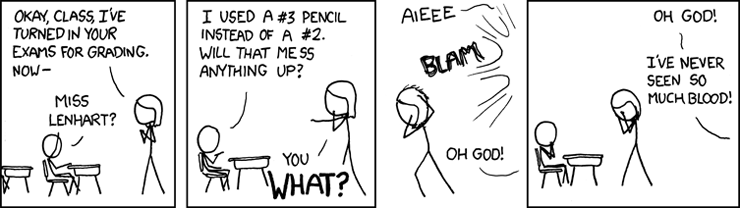
\includegraphics[width=6in]{scantron.png}
	\caption*{Also, after all the warnings about filling in the bubbles completely, I spent like 30 seconds on each one.}
\end{figure}

\end{document}
